\chapter{Numerikus modellezés}
\label{chap:numerical}

Manapság a mérnöki tudományok szinte minden területén teret hódítottak a számítógépes modellezésen alapuló numerikus eljárások, melyek lehetővé teszik a prototípus gyártás és a terméktervezés költséghatékonyságának növelését. Népszerűségük oka a széles körű alkalmazhatóságuk és pontosságuk, mellyel a mérnöki problémák számítógépes modellezését, szimulálását és elemzését teszik lehetővé. A piacvezető szoftverek nemcsak a fizika legtöbb ágát lefedik, de az azok közötti csatolt fizikai jelenségeket is képesek kezelni, például az elektromágneses kölcsönhatás következtében kialakuló Joule-hőt egy ellenállás belsejében vagy a koncentráció változását a diffúzió és a közeg áramlása miatt. A piaci szoftverek a modellezési módszerek és algoritmusok széles palettáján mozognak, kezdve a talán legelterjedtebb végeselem módszerrel, de ezen kívül számos másik metódus is megtalálható, mint például a peremelem módszer\cite{bem}, a véges térfogatok módszere\cite{fvm}, a véges differenciák módszere\cite{fdm} és a momentumok módszere\cite{moment_method}.

Dolgozatomban az elméleti ismeretek bemutatása után ebben a fejezetben a hozzájuk tartozó numerikus szimulációk eredményeit mutatom be. A mérőfej méretezése során több különböző geometriai változat szimulációit készítettem el, azonban a jobb átláthatóság érdekében itt csak a végleges változathoz tartozó eredményeket prezentálom. Az érdeklődő olvasó a további szimulációs eredményeket és ábrákat megtalálja a függelékben szereplő elérhetőségen.

\section{COMSOL Multiphysics}

Kutatómunkám elkészítése során a COMSOL Multiphysics\cite{comsol} programcsomagot használtam, mely egy leginkább végeselem módszeren alapuló parciális differenciálegyenletek megoldására szolgáló program, azonban az utóbbi években a szoftver funkcionalitása jelentősen bővült más formalizmuson alapuló módszerekkel (pl. peremelem módszer). A programcsomag  többféle fizikai szimulációs interfésszel rendelkezik, mint például a kontinuum anyageloszlású testek szimulálására alkalmas Solid mechanics modul, a szilárd testekben tapasztalható hőáramlásra a Heat transfer in solids modul, a termoelasztikus csatolás szimulálásához használt Thermal expansion modul, elektrosztatikai és áramlási terek szimulálásához az AC/DC modul, valamint az elektromos áramok hőhatását szimuláló Joule-heat modul csak hogy néhányat említsek.

A programcsomag, a ma már MathWorks gondozásában álló MATLAB programból nőtte ki magát és a '90-es évek végére lett független\cite{history}, azonban függetlenné válása után is megőrizte a MATLAB szellemiségét. Külön pozitívum, hogy a felhasználóknak lehetőségük van a meglévő fizikai interfészek továbbfejlesztésére (Physics Builder), általuk definiált fizikai egyenletek megadására egy geometriai tartományon (Mathematics module) és a program futása során használt változókat és eredményeket szabadon felhasználhatjuk különféle kiértékelések és fizikai csatolások megvalósítására.

\subsection{LiveLink}

COMSOL Multiphysics alkalmazásánál lehetőségünk nyílik a szoftvert egy lokálisan futtatott szerveren keresztül összekötni más szoftverekkel. Erre egy példa a MATLAB LiveLink\cite{livelink} kapcsolat, mely lehetővé teszi a COMSOL-ban összeállított modellek módosítását, új modellek és szimulációk létrehozását és azok futtatását valamint a szimulációs eredmények utófeldolgozását MATLAB-on keresztül. A LiveLink kapcsolaton keresztül gyakorlatilag a teljes modellezési folyamatot tudjuk irányítani. Ennek köszönhetően lehetőségünk nyílik a modellezési folyamat automatizálására, valamint az utólagos kiértékelés meggyorsítására is. Az automatizálás mértéke, csak a modellt megvalósító kód bonyolultságától és hosszától függ, tehát tetszőleges munkafolyamat megvalósítható LiveLink-en keresztül egy m-fájlból.

Munkám során a LiveLink kapcsolatot elsősorban a geometria létrehozásánál, valamint az utófeldolgozáshoz szükséges definíciók és felületek megalkotásánál használtam. Ezeknél a folyamatoknál a modellezést jelentős mértékben könnyítette az m-fájlban található for ciklusok használata. Ezek nélkül, az egyes szimulációk esetén több száz, felület létrehozása igencsak időigényes lett volna.

\section{Elektrosztatikus szimulációk}
\subsection{Geometria}
\label{sec:El_geometry}

A mérőfej fizikai modellezéséhez meg kellett alkossam annak egyszerűsített geometriai modelljét. A modell megalkotásakor csak az elektrosztatikailag lényeges részekre, vagyis az elektródákra fókuszáltam. A mérőfej mechanikai mozgatását megvalósító MEMS eszköz modellezésétől eltekintettem, hiszen az csak a vizsgált térfogat kis részét tölti ki, valamint az elektrosztatikus vizsgálatok során csak a térrész anyagi összetétele számít, amely így csak kis mértékben tér el a homogéntől. A modelltér méretének meghatározásához egy ponttöltés modellt használtam fel. Ennek részletes számítását \aref{sec:point_charge}. szakaszban tárgyaltam. A mérőfej elektródája és a minta közötti kapacitás meghatározásához a peremelem módszert alkalmaztam, ugyanis így a végtelen kiterjedésű féltér diszkretizációját tudtam helyettesíteni a minta és az elektróda felületének diszkretizációjával. Az így megalkotott elektródaelrendezést  \aref{fig:electrode}. ábrán láthatjuk. Az ábrán az 50 $\mu m$ szélességű elektróda és a hozzá tartozó fókuszáló elektróda geometriai elhelyezkedését láthatjuk a minta felett.

\imgsrc{figures/Simulation/Electrostatic/geometry.png}{A mérő elektróda, a fókuszáló elektróda és a minta elektrosztatikus modellje}{fig:electrode}{0.75}

A minta felületén fellépő koncentrikus körök a diszkretizálás során lesznek hasznosak. A ponttöltéses modellből kiindulva a felületi töltéssűrűség, a minta középpontjából kiindulva radiálisan, 1/r szerint változik, vagyis az elektródától távol a változás mértéke kisebb. A minta felületét ennek megfelelően koncentrikus körívek mentén különböző tartományokra osztottam. Ezekben a tartományokban eltérő méretű diszkretizációs területeket használtam. A szükséges számítási igényt csökkentendő kihasználtam a modell szimmetriáit. A modelltér felosztható lenne nyolc egymással egybevágó vagy tükrözött térrészre, azonban a COMSOL által használt peremelem módszer csak két tengely menti szimmetriát enged meg. A végső modell a teljes geometria negyedét tartalmazza, kihasználva az XZ és YZ síkokra vett szimmetriákat.

\subsection{Diszkretizáció}

A geometriai modell numerikus számítása érdekében annak kontinuum sokaságú pontjait véges számú térrésszel kell közelíteni. Ezt a lépést nevezik diszkretizációnak, vagy szimulációs szaknyelvben hálógenerálásnak, mely az angol meshing szóból származik. A hálógenerálás minősége alapvetően határozza meg a modell és a fizikai valóság összevethetőségét, valamint a modell megoldásához tartozó számítási kapacitás mértékét. Jó minőségű hálók generálásához a szimulációs mérnöknek tisztában kell lennie a modellezett fizikai jelenségekkel és ennek megfelelően kell sűríteni vagy éppen ritkítani a diszkretizációs hálót, a vizsgált fizikai folyamatoknak megfelelően, figyelembe véve a modell geometriájának sajátosságait. Alapvetően a térbeli hirtelen változások lekövetéséhez sűrű hálóra van szükség, míg a lassú változásokhoz elegendő nagyobb méretű diszkretizációs elemek használata is. Az alkalmazott diszkretizációs elemek geometriáját is célszerű a modell geometriájához igazodva választani.

Ennek megfelelően az elektródák felületét négyszög alapú  területekre osztottam, kihasználva ezzel azok négyzetes alakját. Ezzel a diszkretizációval az elektródák felülete kevesebb diszkrét tartományra osztható összehasonlítva a szokásos háromszög alakú térrészekkel. Hálógenerálás során a szoftver igyekszik a háromszöghálókat úgy elhelyezni, hogy a háromszögek torzultsága (szabályos háromszögtől való eltérése) lehetőleg minimális legyen, ennek eredményeként a háromszögháló rendszerint kisebb elemeket használ, így a szükséges elemszám nagyobb.

Ezen elvek mentén kialakított diszkretizációs hálót \aref{fig:mesh_full}. és  \aref{fig:mesh_close}. ábrákon láthatjuk.

\imgsrclr{figures/Simulation/Electrostatic/mesh_full.png}{figures/Simulation/Electrostatic/mesh_close.png}{A teljes geometriát borító háló}{Az elektródákhoz közeli háló}{fig:mesh_full}{fig:mesh_close}{1}{1}

Mint az ábrákon jól látható, az elektróda alatt és közvetlen környezetében egy sűrűbb hálófelosztást használtam, hogy a töltéssűrűség esetleges gyors változásait képes legyen lekövetni a numerikus megoldás. Az elektródától távol a hálóméretet fokozatosan növeltem, így csökkentve a probléma számítási kapacitási igényét.

\subsection{Fizika hozzáadása}

A diszkretizáció elvégzése után elkezdhetjük a modellhez hozzáadni a modellezni kívánt fizikai modulokat. Ezekben a modulokban tudjuk megadni a fizikai jelenség leírásához szükséges paramétereket, megadhatjuk az alkalmazni kívánt szimmetriákat, peremfeltételeket, forrásokat és más fizikákkal történő csatolásokat. Ezeken a modulokon belül lehet beállítani a fizikai modul által használt elemek fokszámát, ami azonos egy hálóelemen belül alkalmazott lokális polinomiális közelítés fokszámával. A fokszámok meghatározásához ismerni kell a fizikai modulban lévő összefüggéseket. Például \aref{eqn:thermomechanical_eqs}. egyenletben szereplő elmozdulásmezőből kétszeres térbeli deriváláson keresztül kapunk egy összefüggést a lokális erősűrűségek, mechanikai feszültségek és gyorsulások között (Newton II. törvénye alapján). Ha az elmozdulásmezőt csak lineáris polinomokkal közelítjük, úgy a kétszeres térbeli deriválás során azonosan nullát kapunk, így az egyenletek diszkretizálása után keletkező egyenletrendszernek nem lesz megoldása. Magasabb fokszámú polinomokat használva a diszkretizáló háló sűrűsége csökkenthető. A háló sűrűsége és az alkalmazott fokszámok közötti optimális arány megadása a szimulációs mérnök feladata.

A COMSOL Multiphysics környezet lehetővé teszi, hogy a modellezni kívánt objektumon több különböző fizikai szimulációt is végrehajtsuk, azonban jelen vizsgálatok során csak az elektrosztatikus peremelem modult használtam (angolul: Electrostatic Boundary Elements). Az elektrosztatikus szimulációjához a modulnak meg kellett adni az elektródák potenciálját, az elektródákat körülvevő homogén közeg relatív dielektromos állandóját, valamint a szimmetriák alkalmazása miatt a szimmetriasíkok pozícióját és a szimmetriák fajtáját (szimmetrikus vagy aszimmetrikus). Ennek eredményeként a program az egyenletrendszer összeállításakor az egyes együtthatók meghatározásakor nemcsak az adott pontbeli töltéseket veszi figyelembe, hanem automatikusan hozzáadja a tükörképek járulékait is.

Az elektródák potenciáljának meghatározásakor kihasználtam az elektrosztatikus tér fizikáját leíró Poisson-egyenlet, valamint a levezetett mennyiségek linearitását is. Ennek eredményeképpen a tér és a térből számítható mennyiségek skálázhatóvá váltak, vagyis elegendő egy tetszőlegesen választott potenciál mellett meghatározni azokat, más potenciálok esete ebből egyszerű skálázással levezethető. Az egyszerűség kedvéért a minta felületét 0 V-os potenciálra választottam, az elektróda felületét 1 V potenciálúnak állítottam be a fókuszáló elektróda esetében pedig a 0 V és az 1 V-os értékekkel is elvégeztem a szimulációkat. Mivel az elektromos tér invariáns a potenciáltér konstanssal vett eltoltjára, így a minta felületi potenciálja nyugodtan megválasztható ebben a formában.

\subsection{A probléma megoldásához használt megoldó motor beállítása}

A probléma számítását végző numerikus megoldó kapcsán is számos beállítási lehetőségünk van. Jelen problémához egy iteratív megoldót választottam, ugyanis a direkt megoldó használatához nem állt rendelkezésemre elegendő memória. Az iteratív megoldók közül a konjugált gradiensen módszer\cite{conjugate} mellett döntöttem. Mivel a megoldás eredményeként előálló töltéseloszlás gyakran irreguláris kilengéseket produkált\footnote{Ennek oka a módszer integrális voltával van összefüggésben, ugyanis ha lokálisan nagy hibával is közelítjük a megoldást az eredmény még lehet globálisan konvergens összességében kis hibával.}, ezért hogy csökkentsem a kilengéseket a megoldóban használt prekondicionáló algoritmust direkt prekondicionálásra állítottam a probléma sűrű mátrixa alapján. A módszer eredményeként a megoldások simasága összemérhető volt a kisebb elemszám esetén végzett direkt megoldásokéval. Mindezek mellett a futásidő is összemérhető volt, azonban a szükséges memória mértéke jóval kevesebb volt az iteratív módszer használatával. A direkt prekondicionálás eredményeként a megoldás általában 1-2 iteráción belül konvergált a megadott ($10^{-12}$) konvergenciaszinten belülire és ehhez átlagosan csak pár percre volt szükség.

\imgsrc{figures/Simulation/Electrostatic/convergence.png}{A szimuláció konvergenciája}{fig:convergence}{0.75}

\Aref{fig:convergence}. ábrán a szimuláció során mérhető konvergenciát ábrázoltam. Látható, hogy a direkt prekondicinálás hatására a megoldás két iterációs lépés után $10^{-24}$-es értéket ért el, így az adott megoldás elhanyagolható hibával elégíti ki a szükséges differenciálegyenleteket. Az szimulációs feladat összetettségének jó mértéke a szabadsági fokok száma, mely ennél a feladatnál kb. 30 000-s nagyságrend környékén mozgott\footnote{A szabadsági fokok száma elsősorban a szimulációs térrész méretétől és a diszkretizáció mértékétől függ.}. Az általam használt számítógépes konfigurációval egy tipikus szimuláció lefuttatása nagyjából pár percet vett igénybe.

\subsection{Utófeldolgozás}

A szimulációk sikeres végeztével megkezdődhetett az adatok utófeldolgozása, melynek során a szimulációs mérnök értelmezi és véleményezi a szimulátor által előállított adatokat, hogy azok megfelelnek-e a fizikai előismereteinek és kvalitatíven elfogadhatóak-e. Az utófeldolgozás során több különböző mennyiséget ábrázoltam és vizsgáltam, hogy egy pontosabb képet kapjak a mérőfej működését befolyásoló hatásokról. A vizsgálat során meghatároztam a felületi töltéseloszlást a minta felszínén a fókuszálás nélkül és azzal együtt, kiértékeltem az elektródák közötti kapacitásokat a mintától mért távolság függvényében, meghatároztam az elektrosztatikus teret a minta és a mérőfej közötti térrészben, valamint az elektrosztatikus tér ekvipotenciális felületeit.

\imgsrclr{figures/Simulation/Electrostatic/unfocused_E_field.png}{figures/Simulation/Electrostatic/focused_E_field.png}{Fókuszálás nélküli elektromos tér}{Fókuszált elektromos tér}{fig:unfocused_E_field}{fig:focused_E_field}{1}{1}

\Aref{fig:unfocused_E_field}. és \aref{fig:focused_E_field}. ábrákon a mérőfej és a minta közötti merőleges síkban ábrázoltam az elektromos potenciál és az elektromos erővonalak eloszlását. Látható, hogy a fókuszálás nélküli esetben a mérőelektróda jelentős szórt térrel rendelkezik, azaz a mérőelektródáról kiinduló erővonalak a minta felületének széles tartományával kauzális kapcsolatban állnak. Fókuszálás hatására az elektromos erővonalak beszorulnak a fókuszáló- és a mérőelektródák közötti térrészbe, ahogy ez \aref{fig:focused_E_field}. ábrán is látható. Az ábrákról az is leolvasható, hogy fókuszált esetben a minta és a mérőfej közötti térrészben az elektromos tér homogénebb, mint a fókuszáló elektróda nélküli esetben. Ennek következtében a kapacitás-távolság karakterisztikák jobban követik az 1/r-es összefüggést, amit egy ideális síkkondenzátortól elvárunk.

A fókuszáló elektróda hatását a minta felületén kialakuló töltéseloszláson is láthatjuk, mely \aref{fig:unfocused_surface_charge}. és \aref{fig:focused_surface_charge}. ábrák mutatnak.

\imgsrclr{figures/Simulation/Electrostatic/unfocused_surface_charge_density.png}{figures/Simulation/Electrostatic/focused_surface_charge_density.png}{Felületi töltéssűrűség eloszlás fókuszáló elektróda nélkül}{Felületi töltéssűrűség eloszlás fókuszáló elektródával}{fig:unfocused_surface_charge}{fig:focused_surface_charge}{1}{1}

Az ábrákon látható, hogy a fókuszálás hatására a felületi töltések a mérőelektródához közeli térrészbe szorulnak be, lekövetve a fókuszáló elektróda négyzetes alakját.

Az elektróda és minta közötti kapacitás együtthatók számításához \aref{sec:focusing}. szakaszban bemutatott módszert alkalmaztam. A szimulációk során több különböző elektródaméretet vizsgáltam. Ezek közös tulajdonsága, hogy geometriájuk egymáshoz hasonló, így az egyetlen paraméterrel jellemezhető. Az általam vizsgált elektródák szélessége: $25\ \mu m,\ 50\ \mu m$ és $75\ \mu m$ volt. Ezen elektródaméretekhez tartozó kapacitás karakterisztikákat \aref{fig:C_z25}., \aref{fig:C_z50}. és \aref{fig:C_z75}. ábrákon láthatjuk.

\imgsrc{figures/Simulation/Electrostatic/c_25.png}{Kapacitás együtthatók $25\ \mu m$-es elektródaszélességnél}{fig:C_z25}{1}
\imgsrc{figures/Simulation/Electrostatic/c_50.png}{Kapacitás együtthatók $50\ \mu m$-es elektródaszélességnél}{fig:C_z50}{1}
\imgsrc{figures/Simulation/Electrostatic/c_75.png}{Kapacitás együtthatók $75\ \mu m$-es elektródaszélességnél}{fig:C_z75}{1}

Az ábrákon jól látható, hogy a kapacitás karakterisztikák jellege hasonló, csak a számított kapacitások értéke tér el. Végül az elektromos tér jobb vizualizációja érdekében elkészítettem az elektródák körül kialakuló elektrosztatikus tér ekvipotenciális felületeit amit \aref{fig:equipot}. ábrán ábrázoltam.

\imgsrc{figures/Simulation/Electrostatic/focused_isosurfaces.png}{Az elektródák körül kialakuló ekvipotenciális felületek}{fig:equipot}{0.75}

\subsection{Analóg méréstechnika}

Az elektródából kinyerhető áramjel feldolgozásához beiktatok egy sönt ellenállást a feszültségforrás és a mérőelektróda közé, ahogy az \aref{fig:circuit}. ábrán látható is. Ezt a kapcsolást felhasználva az elektróda mérőárama egy differenciális feszültségként jelenik meg a sönt ellenálláson. Ezt a feszültséget egy CMOS erősítővel lehet mérni, ahogy azt \aref{fig:control_circuit}. ábrán láthatjuk is. A mérőfejen lévő fókuszálást elvégző elektróda potenciálját a táppal megegyezőre választottam, így a mérőelektróda és a fókuszálás között mérhető $C_{12}$ kapacitás a mérő sönttel párhuzamosan kötődik a kapcsolásban.

A söntellenállás feszültségének mérésével egy elektronikus jelünk áll elő, amit felhasználhatunk a mérés során egy szabályzó jelnek. Ennek köszönhetően a mérőfejet beiktathatjuk egy szabályozókörbe, amivel a rezgő elektróda potenciálját szabályozzuk. Az így kialakult kapcsolás \aref{fig:control_circuit}. ábrán látható. A szabályozási kört felhasználhatjuk a mérőfej áramát minimalizáló feszültségszint megtalálásához. Ehhez a minimalizációhoz egy hibajelet kell előállítani. Mivel a minimalizáció során időfüggvényt mérek, így célszerű a hibajelnek a mért jel átlagos energiáját választani. Egy belépő u(t) jel átlagos energiáját kiszámíthatjuk \aref{eqn:energy} formulával.

\equref{E(t) = \frac{1}{t} \int_0^t u^2(\tau) d\tau}{eqn:energy}

A jel energiaátlagának mérésére többféle lehetőség is előttünk áll. Egyrészt lehetséges \aref{eqn:energy}. formulát analóg áramkörtechnikával direkt megvalósítani egy analóg szorzó, egy integrátor és egy analóg osztó felhasználásával, valamint lehetséges azt egy termikus MEMS segítségével számítani\cite{QTC_MEMS}. A mérőfejet is magában foglaló szabályozási kör vázlatos rajza így \aref{fig:control_circuit}. ábrán bemutatott alakot ölti.

\imgsrc{figures/Simulation/Electrostatic/circuit.png}{A mérőfejhez tartozó szabályozási kör vázlata}{fig:control_circuit}{1}

A kapcsolás jobb oldalán található az elektródákhoz kapcsolódó változó kapacitások, valamint a minta felületi potenciálját jelképező $\phi_\text{ismeretlen}$ feszültségű forrás. $U_\text{ofszet2}$ forrással a minta felületi potenciáljának szintjét tolom el, hogy a mérőelektródáról és a fókuszálásról érkező jelszintek DC értéke megfelelő legyen. Ennek alternatív megoldása a csatoló kondenzátorok alkalmazása, azonban a mérési frekvenciasávhoz szükséges RC tag értékei igen nagyra (néhány pF-os kapacitás és néhány $M\Omega$-os ellenállás) adódnak, melyek a chip felületén sok helyet foglalnak, így célszerűbb a DC csatolás. A mérőfejről érkező jeleket egy differenciálerősítőre kapcsolom, melynek egy lehetséges realizációja az ábrán jelzett áramtükör terhelésű differenciálerősítő. Az erősítő kimeneti jelével hajtom meg az energiaátlag-képző áramköri blokkot, mely lehet tényleges áramkör, vagy MEMS eszköz is. A blokk B-vel jelölt kivezetéséhez kapcsolódó $U_\text{ofszet1}$-es forrással a differenciálerősítő DC feszültségértékét kompenzálom. Az így előálló hibajellel pedig egy szabályzókapcsolást hajtok meg, amely előállítja a szükséges potenciálértéket, mellyel minimalizálható a sönt ellenállás árama.

\section{Termomechanikus szimulációk}

Az elektrosztatikus szimulációkat elvégezve előállíthatóvá vált a mérőfejet meghajtó MEMS eszköz mechanikai specifikációja, mely az elektrosztatikus elektródákat fogja rezgetni a minta felett. A következőkben bemutatom a megtervezett termomechanikus beavatkozó két változatát. A két változat közötti legfőbb különbség a rezgetett platform mérete. Az első változat egyetlen 50 $\mu m$-es elektródát és a hozzá tartozó fókuszáló elektródát képes rezgetni, a rezgetett platform mérete miatt. A második változat nagyobb rezgő platformmal rendelkezik, így a felületén kialakítható négy darab 50 $\mu m$-es elektróda és a hozzájuk tartozó fókuszáló elektródák egy 2x2-es rácsban. A két változatra a továbbiakban 1X és 4X-es jelzővel fogok hivatkozni. A változatok különböző előnyös és hátrányos paraméterekkel rendelkeznek, így ezek összehasonlítása a mérőrendszer jobb megértését és kialakíthatóságát eredményezi. Az 1X-es mérőfej geometriai méretei kisebbek, mint a 4X-es változaté, így a rezonanciafrekvenciája magasabb, ami gyorsabb működést és nagyobb amplitúdójú mérőjeleket eredményez. A 4X-es változat esetében ugyan a működési frekvencia kisebb, azonban a mérés során párhuzamosan négy pontban tudjuk vizsgálni a felületi potenciált, így négyszerezve a letapogatás sebességét.

A következőkben bemutatom a szimulációkhoz készített modellt és annak beállításait függetlenül a mérőfej változataitól (1X vagy 4X), végül pedig a szimulációs eredményeket \aref{sec:thermo_post_process}. szakaszban tárgyalom a két változatot összehasonlítva.

\subsection{Geometria bemutatása}

A mérőfej numerikus modelljének megalkotásakor \aref{sec:El_geometry}. szakaszban leírtakhoz hasonlóan itt is geometriai egyszerűsítésekkel éltem, csökkentve ezzel a szükséges számításigényt. A mérőfej modellezése során csak a teljes geometriájának 1/8-t alkottam meg és szimuláltam le. Ennek magyarázata, hogy a mérőfej 8 eltérő tengely menti tükrözési szimmetriával rendelkezik, így a legtöbb szimuláció során elégséges csak ezt a nyolcad térrészt szimulálni. Ezek a szimmetriatengelyek a mérőfej középpontján átmenő X és Y tengelyekkel párhuzamos egyenesek valamint ezek  $45^\circ$-s elforgatottjaik. A mérőfej teljes geometriáját \aref{fig:mems_geometry_full}. ábrán láthatjuk felülnézetből. A mérőfej közepén lévő négyzetes rész a platform mely a Z tengely mentén fog rezgéseket végezni, a hozzá csatlakozó téglalapok a karok, melyek a rezgő platformot rögzítik és amik tartalmazzak a rezgést keltő fűtőellenállásokat.

\imgsrc{figures/Simulation/Thermomechanic/geometry_full.png}{A teljes mérőfej geometriai modellje felülnézetből}{fig:mems_geometry_full}{0.5}

Az egyetlen szimuláció, mely során a kapott eredmények torzulnak a rezonáns módusok meghatározása során áll fent. A torzulás magyarázata, hogy a mérőfej rendelkezik olyan rezonáns módusokkal is, melyek nem tesznek eleget a már említett tengelyes tükrözési szimmetriáknak. Ennek következtében a redukált geometriával meghatározott módusok csak a lehetséges rezgési módusok részhalmazát fogják képezni. A modellezett geometriát \aref{fig:mems_geometry}. és \aref{fig:mems_si}. ábrákon láthatjuk.

\imgsrclr{figures/Simulation/Thermomechanic/geometry_whole.png}{figures/Simulation/Thermomechanic/geometry_si.png}{A szimulált geometria}{A szimulált szilícium lapka}{fig:mems_geometry}{fig:mems_si}{1}{1}

\Aref{fig:mems_geometry}. ábra a mérőfej teljes geometriájának 1/8-t mutatja. A felső narancssárga réteg a mérőfej bimorf struktúráját adó réz réteg, alatta a szürke színű a szilícium hordozót mutatja. A szimulációk során az elektromos kontaktusok bekötését nem modelleztem, melynek oka, hogy ezeket másik fémréteget használva lehet megvalósítani, ahogy azt később látni is fogjuk. \Aref{fig:mems_si}. ábrán a rézréteg alatt található szilícium lapnak a felülnézeti képét láthatjuk. A kékkel jelölt részek a lapka felületén megvalósított ellenállások körvonalai. A nagyobb ellenállásérték elérése érdekében egy keskeny és hosszú ellenálláscsíkot kell megvalósítani. Ennek egy helytakarékos módszere, hogy az ellenállást párhuzamos szakaszok soros kapcsolásával készítjük el. Ezt a struktúrát meanderes ellenállásnak hívják.

A méretezés során alkalmazott iterációs lépések megkönnyítése érdekében a teljes geometriai modellt paraméteresen alkottam meg, vagyis a teljes geometria alakját néhány paraméter függvényében készítettem el. Ennek következtében egy-egy geometriai méret megváltoztatása csak egy paraméter átírását és a geometriai modellező újrafuttatását igényelte ezzel nagyban meggyorsítva a méretezési feladatot. Ilyen geometriai paraméterek voltak a karok hosszai, azok szélessége, a platform szélessége és ehhez hasonló paraméterek. A mérőfejek végleges geometriai méreteit és a modellezés során felhasznált paramétereket \aref{tab:compare}. táblázatban láthatjuk.

\subsection{Diszkretizáció}

A numerikus szimulációk elvégzéséhez a következő szükséges lépés a modell geometriájának diszkretizációja. A diszkretizációs háló létrehozásakor kihasználtam a modell geometriai adottságait, így a középső platformot tartó téglatest alakú tartó karokat téglatestekkel hálóztam be, míg a platformot magát prizma alakú elemekkel osztottam fel. A diszkretizáció során ügyeltem a karok keresztmetszeti felosztásának finomra állítására, így a rezgések során elegendő diszkrét felületelem található bennük, hogy a keresztmetszeti változásokat pontosan tudják lekövetni. Ilyen keresztmetszeti változások a karok keresztmetszetében ébredő nyomó- és szakító feszültségek, melyek a rezgések során keletkeznek és folyamatosan változnak az idő függvényében.

\imgsrclr{figures/Simulation/Thermomechanic/mesh_whole.png}{figures/Simulation/Thermomechanic/mesh_close.png}{Az egész geometriát borító diszkretizációs háló}{A karok keresztmetszeti diszkretizációs hálója}{fig:mesh_whole}{fig:mesh_arms}{1}{1}

\Aref{fig:mesh_whole}. és \aref{fig:mesh_arms}. ábrán látható az általam alkalmazott diszkretizációs háló. Az ábrákról jól látható a karok felületén és keresztmetszetén alkalmazott sűrű felosztás, míg a platform felületén sokkal ritkább felosztás is megengedhető, ennek oka, hogy a platform felülete jelentős deformációt nem fog szenvedni a rezgés során felerősített rezonanciamódusban rezegve.

A mérőfej hálózását megkönnyítendő úgynevezett húzott (vagy angolul swept) hálózást alkalmaztam. Ennek folyamán először a szilíciumlapka és a réz réteg határfelületén készítettem el a felületi diszkretizációs hálót, a karokon négyszögletes a platformon háromszögű elemeket használva. A térfogati diszkretizáció elérésére az így kialakított felületi hálót eltoltam a Z tengely mentén és az általam megadott darabszámú diszkretizációs elemet hoztam létre a modell térfogatában.

\imgsrc{figures/Simulation/Thermomechanic/mesh_resistor.png}{A szilíciumlapka felületén kialakuló diszkretizációs háló}{fig:mesh_resistance}{0.5}

A karok felületén látható hálózási egyenetlenségek a szilícium hordozó felületén elhelyezett ellenállások geometriája miatt van, ahogy az \aref{fig:mesh_resistance}. ábrán látható is. A hálózás során a diszkretizációt végző algoritmus igyekszik az általam beállított mérettartományú elemekkel lefedni a felületet, így az elemek alakja torzul, hogy beférjenek a felületet határoló tartományokba.

\subsection{Fizika hozzáadása}

A diszkretizáció után következhetett a szükséges fizikai csatolásokat tartalmazó modulok modellhez adása. Az elektrosztatikus szimulációkkal szemben itt több különböző fizikai interfész került felhasználásra. A statikus hőtágulás szimulálásához szükség volt a termikus és mechanikus szimulációkat tartalmazó interfészekre, ezek a COMSOL Multiphysics-ben a Heat Transfer in Solids és Solid Mechanics néven érhetők el. A modulok külön-külön szimulálják a termikus és mechanikai alrendszerek működését, annak érdekében, hogy a két fizikai mező (hőmérséklet és elmozdulás) között kapcsolatot létesítsünk egy fizikai csatolást kell megvalósítani. Ehhez alapvetően több lehetőség állt rendelkezésemre. Az egyik lehetőség, hogy a beépített dedikált hőtágulás interfészt használom fel, azonban a későbbiekben csatolandó nagyfrekvenciás hőtágulást ez az interfész nem támogatta, így ez a csatolási mód számomra nem volt praktikus. Egy másik lehetőség a csatolás létrehozásában a Solid Mechanics modulon belül található lineáris rugalmassággal rendelkező alegységhez hozzáadni a hőtágulást. A módszer előnye, hogy az így hozzáadott modul csak a hőmérsékleti mezőt és a referencia hőmérsékletet kéri, mint bemenő adat. A fizikai interfész számára megadott kényszerek \aref{fig:DC_heat_settings}. ábrán láthatók.

A rezonáns viselkedés vizsgálatához felhasználtam a már korábban hozzáadott Solid Mechanics modult. A korábban beállított paramétereken és kényszereken nem volt szükséges változtatni, hiszen a különböző beállítási lehetősége a numerikus probléma megoldó motorjaiban külön-külön kikapcsolhatók. Hasonlóan a tranziens hőtágulás számításához itt sem volt szükség új modul hozzáadására csak a meglévők módosítására egy időfüggő gerjesztő mennyiség hozzáadásával.

A nagyfrekvenciás hőterjedés számításához szükséges volt még egy új modul hozzáadása a szimulációs környezethez. Mivel a COMSOL Multiphysics nem rendelkezik állandósult hőterjedés számítására alkalmas modullal, így azt nekem kellett összeállítani. Szerencsére a COMSOL támogatja az új fizikai interfészek és modulok fejlesztését, valamint a szokványostól eltérő matematikai problémák megoldását is. Ennek következtében a programon belül lehetősége van a szimulációs mérnöknek egy általános PDE (Partial Differential Equations, avagy parciális differenciál egyenletek) modul hozzáadására és a PDE együtthatóinak a definiálására a modellezni kívánt problémának megfelelően. Az általános PDE modulon kívül a szokványos differenciálegyenletekhez is léteznek egyszerűsített modulok, ilyenek a Laplace-, Poisson-, diffúziós- vagy éppen a Helmholtz-egyenlet modul. \Aref{sec:sinusoidal}. szakaszban levezetett állandósult állapotot leíró differenciál egyenletrendszer hőterjedést befolyásoló tagja pontosan egy Helmholtz-egyenlet, így a szimulálásához a Helmholtz-egyenlet modult adtam hozzá a modellhez. A PDE együtthatóinak beállítása után a COMSOL képes volt a hőterjedés állandósult állapotának szimulálására. A beállítások ellenőrzéséhez összehasonlítottam a dedikált hőterjedést számoló modul és az általam implementált modul eredményeit nagyon kicsi frekvencián, mellyel a statikus hőterjedést közelítettem. Az összehasonlítás eredményeiből láttam, hogy a két modul azonos megoldásokat produkált. A Helmholtz modul beállításait és kényszereit \aref{fig:Helmholtz}. ábrán láthatjuk.

\imgsrclr{figures/Simulation/Thermomechanic/DC_heat_expansion_settings.png}{figures/Simulation/Thermomechanic/Helmholtz_settings.png}{A termomechanikus interfészek beállításai és kényszerei}{A Helmholtz modul beállításai és kényszerei}{fig:DC_heat_settings}{fig:Helmholtz}{0.5}{0.5}

A mérőfej kitérésének kapcsoláson belüli méréséhez felhasználom \aref{sec:piezo}. szakaszban bemutatott piezorezisztív méréstechnikát. A méréséhez szükséges a mérőfejet gerjesztő ellenállások karakterizációjára a kitérés függvényében. A karakterisztikák szimulálásához szükségem volt a piezorezisztív csatolás hozzáadásához a modellemhez. Ennek a csatolásnak a modellezéséhez a COMSOL rendelkezik beépített modullal, így ezeket fel tudtam használni. A piezorezisztív modul beimportálásakor a COMSOL automatikusan hozzáad egy Solid Mechanics modult, egy Electric Current Single Layer Shell és egy Piezoresistive Effect Boundary Currents modult a modellhez. Az Electric Current Single Layer Shell modul a felületi rétegekben folyó áramokat szimulálja. A felületi áramok szimulációja az általam megkívánt alkalmazáshoz elfogadható közelítést jelent, hiszen a kész mérőfejben is a felületre integrált poliszilícium ellenállások fogják biztosítani a szükséges hőteljesítményt. A Piezoresistive Effect Boundary Currents modul pedig ezeknek a felületi áramok mechanikai feszültségekkel történő csatolását valósítja meg \aref{eqn:piezo_coupling}. egyenletben leírtak szerint. A modul beállításait és kényszereit \aref{fig:piezo_settings}. ábrán láthatjuk.

\imgsrc{figures/Simulation/Thermomechanic/piezo_settings.png}{A piezorezisztív interfész beállításai és kényszerei}{fig:piezo_settings}{0.25}

\subsection{A probléma megoldásához használt megoldó motor beállítása}

A fizikai interfészek konfigurálása után beállítottam a vizsgálatokhoz szükséges szimulációs motorokat kihasználva a fizikai csatolások jellemzőit. A statikus hőtágulás számításához egy állandósult állapotot kellett megtalálni, így ehhez egy stacionárius megoldót használtam. A hőtágulás szimulációjánál csak egy egyirányú fizikai csatolást kellett figyelembe vegyek, vagyis a termikus mező hatását a mechanikusra, ennek következtében a fizikai interfészek között lehetőségem volt szegregált szimuláció használatára (angolul segregated). A módszer lényege, hogy egyetlen nagy méretű csatolt egyenletrendszer helyett a fizikai hatásokat egymás után veszem figyelembe. A hőtágulás esetén meghatároztam először a termikus mezőt, majd a hőtágulási együtthatón keresztül ez a mező egy adott alakváltozást gyakorolt a mechanikai elmozdulásmezőre, mely a deformációjával és a megjelenő mechanikai feszültségekkel reagált erre. Mivel csak egyirányú csatolást vettünk figyelembe, így a mechanikai alakváltozás hatása nem lett belekalkulálva a termikus mezőbe, így ezen két mező megoldását egymás után többször kell ismételni közben felhasználva az előző megoldás értékeit. Ezzel a módszerrel a megoldó néhány iteráción belül megfelelő eredményt produkált. Ennek a módszernek az előnye, hogy lehetőségünk nyílt a fizikai interfészeket külön modellezni, ezáltal jelentősen csökkent a szükséges számításigény. \Aref{fig:segregated_convergence}. ábrán a statikus hőtágulás számításakor elért konvergencia látható.

Egy egyszerű számpéldán végigkövethetjük a módszer számításigényét a teljesen csatolt megoldóhoz képest. Tételezzük fel, hogy egy adott diszkretizáció mellett százezer mintavételi pontunk van. Ebben a százezer pontban szeretnénk meghatározni a hőmérséklet értékét, ehhez százezer egyenlet szükséges. Az elmozdulásmező megadásához ennek háromszorosa kell, hiszen az elmozdulás vektoriális mennyiség, így meg kell adni az x, y és z koordinátáját az elmozdulásnak minden mintavételi pontban. Ennek következtében a teljesen csatolt leírás négyszázezer ismeretlent tartalmaz, míg a szegregált csak száz- plusz háromszázezret. Az egyenletrendszerek megoldásához az őket leíró együtthatómátrixot, vagy rendszermátrixot kell invertáljuk. Egy NxN-es négyzetes mátrix invertálása O(N!) számú lépést igényelne, ha a determinánsa segítségével szeretnénk azt meghatározni, azonban, ha mátrixfelbontásokat alkalmazunk akkor csak O($N^3$) lépés kell. A teljesen csatolt probléma megoldásához tehát 6,4 $10^{16}$ lépés szükséges, míg a szegregált rendszerhez elegendő 2,8 $10^{16}$. Látható, hogy a lépésszám kb. felére csökkent hasonlóan a szükséges memória is kb. a felére csökkenthető. Ha tehát a szegregált megoldónak két iteráció szükséges a probléma megoldásához, akkor ezt a módszert használva gyorsabban és kevesebb memória árán kaptuk meg a csatolt rendszer megoldását.

\imgsrc{figures/Simulation/Thermomechanic/segregated_solver.png}{A szegregált megoldómotor konvergenciája}{fig:segregated_convergence}{0.5}

A mechanikai szerkezet rezonáns módusainak meghatározásához a COMSOL beépített sajátérték-probléma megoldómotorját használtam fel. A módszer alapja, hogy a megoldást $\vec{u}(\vec{r})e^{j\omega t}$ alakban keressük. Ekkor az időbeli deriváltak $j\omega$-val való szorzássá egyszerűsödnek, így a homogén differenciálegyenlet rendszer átalakul egy algebrai egyenletrendszerré a $e^{j\omega t}$-s tagokkal történő egyszerűsítés után. Ezt - az általában nemlineáris - egyenletrendszert ezután egy sajátérték problémának tekinthetjük, melyben a sajátértékek a rezonáns frekvenciák, míg a sajátvektorok az adott rezonanciafrekvenciához tartozó módusok vagy más szóval lengésképek. A hőtágulás következtében létrejövő deformáció miatt a deformálódott rendszer rezonanciafrekvenciái eltolódnak a referencia konfigurációéhoz képest. Ennek a hatásnak a kompenzálásához a sajátprobléma megoldójának beállításainál a deformálódott konfigurációt adtam meg, mint linearizálási pont. Ennek következtében a megoldó a hőtáguláson átesett konfigurációt linearizálja és ebben a munkapontban számított lineáris modellnek határozza meg a rezonanciafrekvenciáit és lengésképeit.

A nagyfrekvenciás hőtágulás számításához egy frekvenciatartománybeli gerjesztett állapotot kellett számoljak, ehhez pedig a rendelkezésemre állt a COMSOL beépített megoldómotorja a Frequency Domain Perturbation motor. A motor a rezonáns megoldóhoz hasonlóan egy adott munkapontban linearizált modellt gerjeszt egy általam megadott frekvenciájú mennyiséggel. Ennél a szimulációnál a mechanikai interfészben a nagyfrekvenciás hőtáguláshoz használt modult kapcsoltam be, ami a hőmérséklet eloszlást a Helmholtz-egyenletből veszi. Ez a megoldómotor az állandósult állapothoz hasonlóan egy lineáris (vagy nemlineáris) algebrai egyenletet old meg.

A mérőfej működését verifikáló tranziens szimulációkhoz egy tranziens megoldót használtam fel. Ez a megoldómotor a rendszert leíró PDE-t numerikus integrálás segítségével oldja meg adott kezdeti-értékből kiindulva. A stabilitás érdekében a megoldóban a Hátralépő-Euler módszert használtam fel, és az állandósult állapot eléréséhez igen sok periódust szimuláltam.

A piezorezisztív hatás szimulálásához szintén egy stacionárius megoldót használtam fel a statikus hőtáguláshoz hasonlóan. Ezen szimulációk során a mérőfej platformjának kitérését határoztam meg mint kezdeti gerjesztés, ebből egy szegregált megoldóval meghatároztam a mechanikai feszültségeket és ebből a kiadódó ellenállásértékeket.

\subsection{Utófeldolgozás}
\label{sec:thermo_post_process}

A szimulációk végeztével elkezdtem a szükséges utófeldolgozási lépéseket, vagyis a számomra értékes numerikus értékek meghatározását, a karakterisztikák szerkesztését és a különböző táblázatok elkészítését. Ehhez a munkához elsősorban a COMSOL beépített eredménykiértékelő módszereit használtam fel.

A termomechanikus modellek eddig bemutatott ábrái és beállításai univerzálisak voltak, azaz mindkét méretezett mérőfejhez kvalitatíven illeszkedtek. A továbbiakban az 1X-es és 4X-es mérőfejváltozat eredményeit mutatom be. Az ábrákon csak az 1X-es változatot tüntettem fel, hiszen a 4X-es változat minden szimuláció során hasonló eredményeket produkált, csak a numerikus értékekben tértek el. Ezeket a numerikus értékeket a fejezet végén lévő \aref{tab:compare}. táblázatban összegzem és hasonlítom őket össze.

\subsubsection{Statikus hőtágulás}

A statikus hőtágulás szimulációjának eredményeként előáll a felületi hőmérséklet eloszlás, valamint a hőmérséklet által gerjesztett hőtágulás is, ezeket \aref{fig:DC_temp}. és \aref{fig:DC_expansion}. ábrákon láthatjuk.

\imgsrc{figures/Simulation/Thermomechanic/DC_heat_distribution.png}{Statikus hőmérsékleti eloszlás a mérőfej felületén}{fig:DC_temp}{0.5}
\imgsrc{figures/Simulation/Thermomechanic/DC_heat_expansion.png}{Statikus hőtágulás hatása a mérőfejre}{fig:DC_expansion}{0.6}

Az ábrákon jól látható, hogy a hőmérséklet eloszlás és mechanikai deformáció a mérőfej közepe felé haladva monoton nő, igazodva a fizikai intuícióhoz. A két mérőfejváltozat szimulációja kvalitatíve azonos eredményeket ad vissza, így azokat külön ábrákon nem tüntetem fel. Az eredmények kvantitatív összehasonlíthatóságáért meghatároztam a mérőfejem mérhető maximális hőmérsékleti értéket, valamint a Z irányú maximális deformáció mértékét. Ezeket az eredményeket \aref{tab:DC_expansion}. táblázatban összegeztem a mérőfejet meghajtó ellenállás áramerősségének függvényében. A táblázatban lévő hőmérsékleti értékek 20 $^\circ C$ mellett voltak szimulálva.

\begin{table}[!ht]
    \centering
    \footnotesize
    \makebox[\textwidth]{
    \begin{tabular}{@{}cccccc@{}}
        \toprule
        & \multicolumn{2}{c}{\textbf{1X}} & & \multicolumn{2}{c}{\textbf{4X}} \\
        \cmidrule{2-3} \cmidrule{5-6}
        & \textbf{Felületi} & \textbf{Z irányú} & & \textbf{Felületi} & \textbf{Z irányú} \\
        \textbf{Áramerősség} & \textbf{hőmérséklet} & \textbf{kitérés} & &  \textbf{hőmérséklet} & \textbf{kitérés} \\
        \textbf{(mA)} & \textbf{maximuma ($^\circ C$)} & \textbf{maximuma (nm)} & & \textbf{maximuma ($^\circ C$)} & \textbf{maximuma (nm)} \\
        \hline
        0,5 & 20,51 & 14 & & 20,18 & 16 \\
        1 & 22,07 & 58 & & 20,72 & 64 \\
        2 & 28,28 & 235 & & 22,88 & 257 \\
        5 & 71,78 & 1451 & & 38,05 & 1599 \\
        10 & 227,14 & 5621 & & 92,2 & 6306 \\
        \bottomrule
    \end{tabular}}
    \caption{Statikus hőtágulás mértéke különböző áramerősségek mellett}
    \label{tab:DC_expansion}
\end{table}

A táblázatból látható, hogy a két mérőfejváltozat közül az 1X-es változaton nagyobb hőmérséklet változás mérhető adott áramerősség mellett. Ennek oka, hogy az 1X-es változat keskenyebb, így a termikus ellenállása nagyobb, mint a 4X-es változaté, valamint a felületén kialakított ellenállásértékek nagyobbak a keskenyebb csíkszélesség miatt. Ugyanakkor a 4X-es változat kisebb hőmérséklet változás mellett is hasonló kitéréseket ér el mivel a karok hosszabbak, így kisebb hosszegységre eső gerjesztés esetén is nagyobb az összesített kitérés értéke.

\subsubsection{Rezonáns viselkedés vizsgálata}

A mechanikai sajátproblémát megoldva megkaphatók a mérőfej rezonanciafrekvenciái és a hozzájuk tartozó módusok vagy lengésképek térbeli eloszlásai. A redukált geometria alkalmazása miatt (kihasználva a mérőfej szimmetriáit) a kiadódó lengésképek torzítottak lesznek, hiszen azok a rezgési módusok melyek nem felelnek meg a támasztott szimmetriáknak, nem jelennek meg a megoldások között. Ilyen rezgési módus tud lenni a mérőfej forgása az XY síkban, hiszen ez a mozgás antiszimmetrikus peremfeltételt kíván meg az X és Y tengelyekkel párhuzamos egyenesek mentén. A mérőfej két változata között ismét csak kvantitatív különbségek vannak, így a kiadódó lengésképeket csak az 1X-es változat esetén ábrázolom. Az eltérő rezonanciafrekvenciákat \aref{tab:resonant}. táblázatban összesítem.

\imgsrclr{figures/Simulation/Thermomechanic/resonant_1.png}{figures/Simulation/Thermomechanic/resonant_2.png}{Az első rezonanciafrekvenciához tartozó lengéskép}{A második rezonanciafrekvenciához tartozó lengéskép}{fig:resonant_1}{fig:resonant_2}{1}{1}

\Aref{fig:resonant_1}. ábrán látható a mérőfej első rezonanciafrekvenciájához tartozó lengéskép, míg \aref{fig:resonant_2}. ábrán a második rezonanciafrekvenciához tartozó lengéskép. Az ábrákon jól látható, hogy a rezonáns módusok hasonlítanak egy kifeszített kör alakú membrán szimmetrikus lengésképeihez\cite{bessel}.

\begin{table}[!ht]
    \centering
    \makebox[\textwidth]{
    \begin{tabular}{@{}ccc@{}}
        \toprule
        & \textbf{1X} & \textbf{4X} \\
        \textbf{Rezonanciafrekvencia} & \textbf{Rezonanciafrekvencia} & \textbf{Rezonanciafrekvencia} \\
        \textbf{sorszáma} & \textbf{(kHz)} & \textbf{(kHz)} \\
        \hline
        1. & 151,54 & 52,633 \\
        2. & 848,48 & 305,99 \\
        3. & 1670,8 & 471,90 \\
	    4. & 2560,3 & 847,22 \\
        5. & 3804,1 & 1251,7 \\
        \bottomrule
    \end{tabular}}
    \caption{A mérőfejek első öt rezonanciafrekvenciája}
    \label{tab:resonant}
\end{table}

A táblázatból látható, hogy a 4X-es mérőfej kb. harmadakkora rezonanciafrekvenciákkal rendelkezik, mint az 1X-es változat. Ennek oka a nagyobb geometriai méretek, melyek kétszeresen fejtik ki a hatásukat. Egyrészt a hosszabb karok lágyabbak, vagyis rugóállandójuk kisebb, másrészt a nagyobb méret miatt a 4X-es mérőfej tömege is nagyobb, így mindkét hatás a rezonanciafrekvencia csökkenésével fog járni.

\subsubsection{Nagyfrekvenciás hőtágulás}

A nagyfrekvenciás viselkedés optimalizálásáért a méretezés során a rezonáns lengéskép térfogati alakváltozásából indultam ki, mely megadja hogy a termikus gerjesztéssel a mérőfejet, mely pontokon és milyen fázisokkal kell gerjeszteni. Ennek következtében a mérőfej karjain nem egy darab főtőellenállást helyeztem el, hanem kettőt a karok hossza mentén 6:4-es arányban. Ennek magyarázat, hogy a számomra értékes első rezonanciafrekvenciához tartozó rezgés során a karok felülete nem azonos feszültségállapotban van. \Aref{fig:resonant_1}. ábrán jól látható módon a karok S alakú deformációt szenvednek a rezgés során, így a rezgés egyik szélsőértékénél a karok felső oldala a mérőfejhez közel nyomó-, míg attól távol szakító feszültséget tapasztal és ezzel ellentétes állapotok érzékelhetőek a karok alsó oldalán. Ennek az optimalizációnak köszönhetően azonos termikus gerjesztés mellett háromszoros rezgési amplitúdót kapunk.

A mérőfejek az előzőekhez hasonlóan közel azonosan viselkednek, így az ábrákon csak az 1X-es változat eredményeit tüntetem fel. A mérőfejek nagyfrekvenciás rezgése \aref{fig:AC_vibration}. ábrán láthatók a rezgés különböző fázisaiban. Az első oszlopban látható a szilíciumlapka felületén kialakuló nagyfrekvenciás hőmérséklet eloszlás, a második oszlopban pedig a hőmérséklet eloszláshoz tartozó deformáció. A két mérőfej által produkált amplitúdóit \aref{tab:AC_amplitudes}. táblázatban összegeztem.

A modell eredményéül előálló pár száz $\mu m$-s elmozdulások a linearizált modell és a kis csillapítás következményei. A valóságban a légellenállás, a mechanikai nemlinearitások és az advektív hőfluxus is befolyásolja ezeket az értékeket, ezért szükséges a mérőfej tranziens verifikációja és a gyártás utáni verifikációja.

\begin{table}[!ht]
    \centering
    \begin{tabular}{@{}cc@{}}
        \toprule
        \textbf{Mérőfej változat} & \textbf{Z irányú amplitúdó ($\mu m$)} \\
        \hline
        \textbf{1X} & 250 \\
        \textbf{4X} & 350 \\
        \bottomrule
    \end{tabular}
    \caption{A linearizált hálózat nagyfrekvenciás hőtágulásának amplitúdói}
    \label{tab:AC_amplitudes}
\end{table}


\renewcommand{\arraystretch}{0.6}
\begin{figure}[!ht]
    \centering
    \begin{tabular}{@{}cc@{}}
        \resizebox{0.42\linewidth}{!}{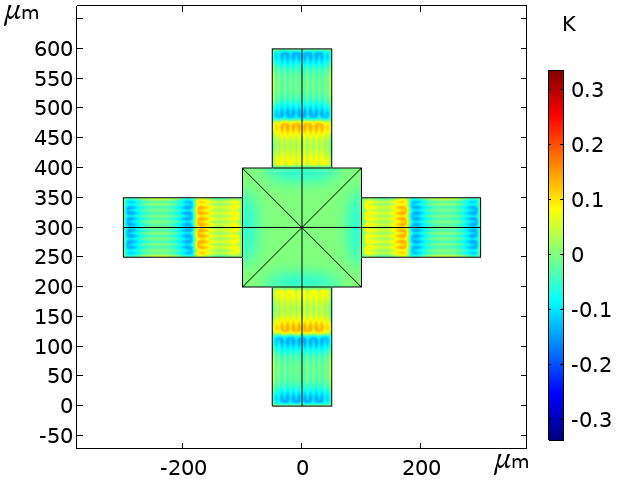
\includegraphics{figures/Simulation/Thermomechanic/AC_temp_field1.png}} &
        \resizebox{0.55\linewidth}{!}{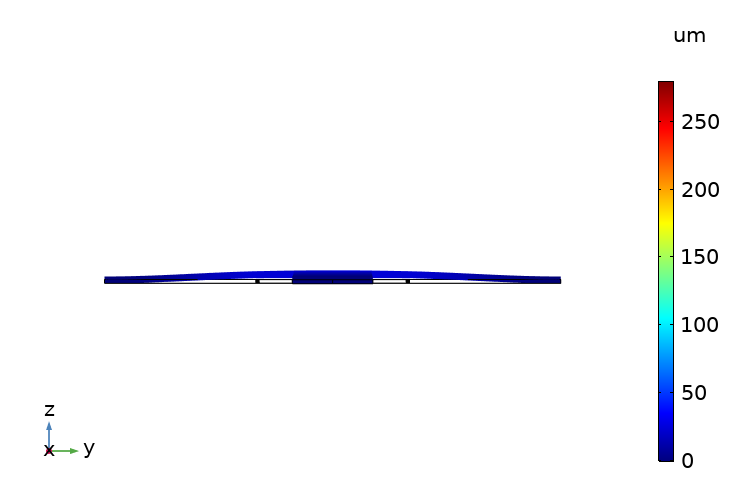
\includegraphics{figures/Simulation/Thermomechanic/Displacement_side1.png}} \\
        \resizebox{0.42\linewidth}{!}{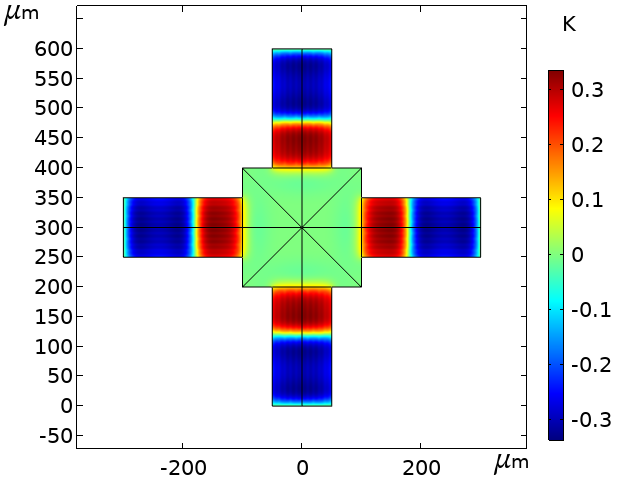
\includegraphics{figures/Simulation/Thermomechanic/AC_temp_field2.png}} &
        \resizebox{0.55\linewidth}{!}{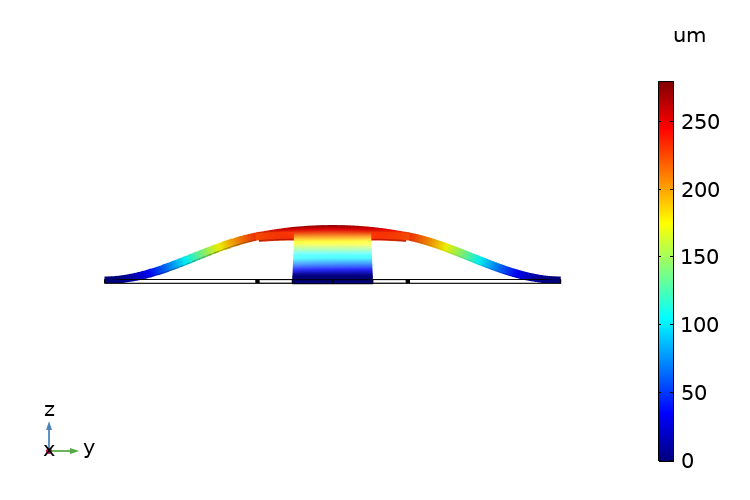
\includegraphics{figures/Simulation/Thermomechanic/Displacement_side2.png}} \\
        \resizebox{0.42\linewidth}{!}{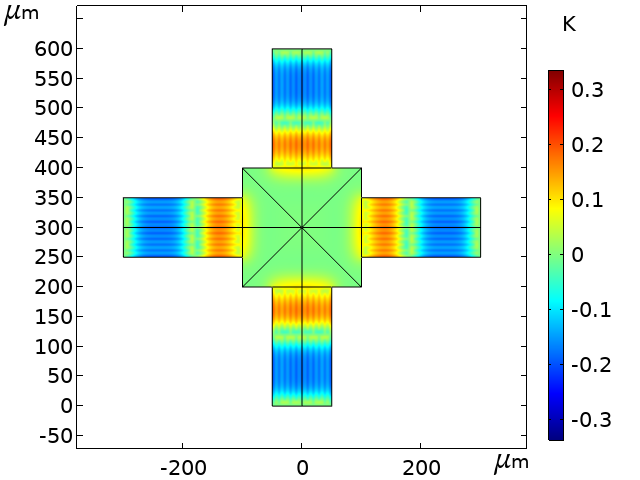
\includegraphics{figures/Simulation/Thermomechanic/AC_temp_field3.png}} &
        \resizebox{0.55\linewidth}{!}{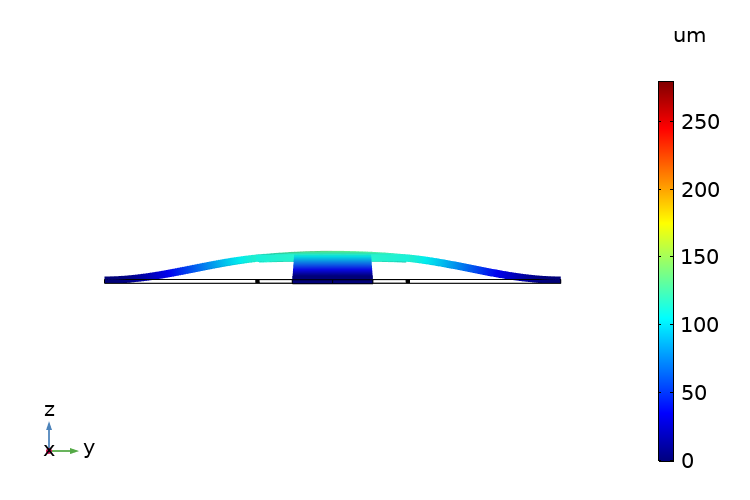
\includegraphics{figures/Simulation/Thermomechanic/Displacement_side3.png}} \\
        \resizebox{0.42\linewidth}{!}{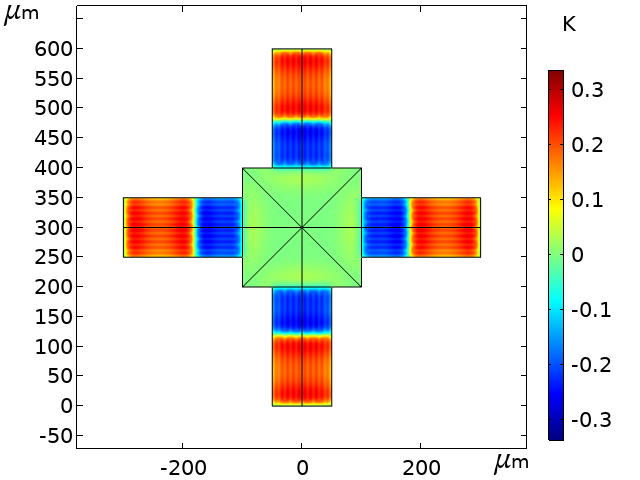
\includegraphics{figures/Simulation/Thermomechanic/AC_temp_field4.png}} &
        \resizebox{0.55\linewidth}{!}{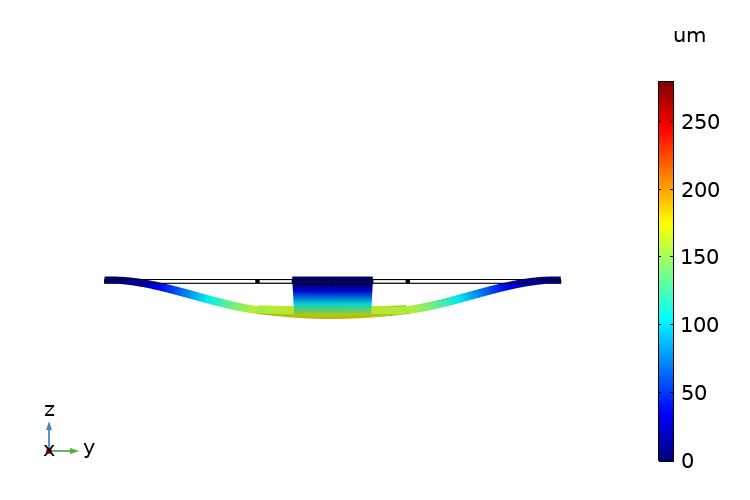
\includegraphics{figures/Simulation/Thermomechanic/Displacement_side4.png}} \\
    \end{tabular}
    \caption{A nagyfrekvenciás hőtágulás okozta rezgés különböző fázisai}
    \label{fig:AC_vibration}
    \vfill
\end{figure}


\subsubsection{Piezorezisztív hatások}

A termomechanikus viselkedés vizsgálata érdekében a mérőfej mozgását a termikus gerjesztést megvalósító ellenállások segítségével vissza is tudjuk mérni kihasználva a piezorezisztív hatást. A mérés elvégzéséhez ismerni kell a mérőfej ellenállás-kitérés karakterisztikáit amikből visszaszámolható a Z irányú kitérés értéke. Ezeknek a karakterisztikáknak a meghatározását a COMSOL Multiphysics beépített piezorezisztív csatolásának segítségével határoztam meg. A szimulációk során a mechanikai rendszernek előírtam a Z irányú kitérését és ebből meghatároztam a karok felületén kialakuló mechanikai feszültségek állapotait. Ezeket az eredményeket felhasználva meghatározható a termikus gerjesztést megvalósító ellenállások mechanikai feszültséggel terhelt ellenállása. Ezeket a karakterisztikákat \aref{fig:piezores_1}. és \aref{fig:piezores_2}. ábrákon mutatom be.

\imgsrclr{figures/Simulation/Thermomechanic/Piezo_1.png}{figures/Simulation/Thermomechanic/Piezo_2.png}{Az 1X mérőfej ellenállásainak ellenállás-kitérés karakterisztikái}{Az 4X mérőfej ellenállásainak ellenállás-kitérés karakterisztikái}{fig:piezores_1}{fig:piezores_2}{1}{1}

A szimulációk során lineáris piezorezisztív hatást és lineáris mechanikai összefüggéseket használtam fel, így a kiadódó karakterisztikák egyenesnek adódtak, ahogy azt el is várhatjuk. Ha a szimulációk során a Green-Lagrange-féle alakváltozási tenzorokat használom fel a mechanikai deformációjára, akkor a kiadódó karakterisztikák parabolikusak lesznek, ahogy azt a másodfokú mechanikai egyenletekből és a lineáris piezorezisztív hatásból várnánk.

A kiadódó karakterisztikák jól tükrözik a két ellenállás alatt kialakuló ellentétes mechanikai feszültségállapotokat, hiszen a kitérés folyamatos növelésével az R1-es ellenállás értéke növekszik, indikálva ezzel a növekvő nyomófeszültség\footnote{A szilárdságtanban a szakító feszültségek előjele pozitív és a nyomófeszültségé negatív, így a negatív piezorezisztív együtthatóval együtt egy pozitív együtthatót adnak.} értéket valamint az N adalékolású szilícium negatív piezorezisztív együtthatóját\cite{piezoresistivity}. Az R2 ellenállásnál a szakítófeszültségek növekednek, így az ellenállás karakterisztikája csökkenő tendenciát mutat.

\subsubsection{Tranziens verifikáció}

A mérőfej tervezésének végső fázisa a megtervezett mérőfej verifikációja. Erre a lépésre azért van szükség, mert a tervezés korábbi stádiumaiban több közelítéssel és elhanyagolással is éltem. Ezek között szerepel például a hőtranszport egyenletben elhanyagolt advektív tag. A verifikáció elvégzéséhez összeállítottam a geometriát és hozzáadtam a COMSOL által biztosított mechanikai és hőtranszport modult. Ezután elvégeztem egy stacionárius szimulációt, a DC komponensek meghatározásához. Ezzel a lépéssel a tranziens szimulációhoz megadhatom az így kiszámolt értékeket, mint kiindulási érték, ezáltal csökkentve a tranziens szimuláció számításigényét, hiszen nem kell megvárni míg beáll az állandósult állapot.

Ezután következett a csatolt fizikai tranziens szimuláció, mely során az állandósult DC állapotból kiindulva időtartományban szimuláltam a mérőfejet. A szimuláció kezdeti szakaszában látható a rezonancia jelensége, hiszen a kitérés amplitúdója az idővel lineárisan növekszik, ahogy az \aref{fig:trans_small}. ábrán látható is. A szimuláció későbbi szakaszában a nemlineáris jelenségek miatt megjelentek a felharmonikusok is a megoldásban, melyet \aref{fig:trans_large}. ábrán láthatunk az amplitúdó modulációjából. Végül a teljes berezgés kitérés-idő diagramját \aref{fig:trans_full}. ábrán láthatjuk. Az ábráról jól látható, hogy a mérőfej kitérései kb. 10 $\mu m$-es nagyságrendnél állandósulnak.

\imgsrc{figures/Simulation/Thermomechanic/transient_full.png}{Tranziens verifikációs szimuláció}{fig:trans_full}{0.8}
\imgsrclr{figures/Simulation/Thermomechanic/transient_small.png}{figures/Simulation/Thermomechanic/transient_large.png}{Kezdeti rezgések lineárisan változó amplitúdói}{Amplitúdó moduláció a felharmonikusok miatt}{fig:trans_small}{fig:trans_large}{0.75}{0.75}

\subsection{Mérőfejváltozatok összehasonlítása}

A megtervezett mérőfejek geometriai adatait és fontosabb szimulációs adatokat \aref{tab:compare}. táblázatban összegeztem. A méretezés során az elektrosztatikus szimulációk eredményéül előálló 50 $\mu m$-es elektródaméretet vettem alapul. Ennek következtében a mérőfejből két különböző változatot készítettem el és szimuláltam le. A két változat között a rezgetett platform mérete az elsődleges megkülönböztető paraméter. Az első változat geometriai mérete 1 mérőelektróda elhelyezését teszi lehetővé, míg a második változatra 4 mérőelektróda helyezhető el egy 2x2-es rácsban. Ebből a parametrikus különbségből származtattam a változatok megnevezéseit is (1X és 4X-es változat).

A platformok méretének különbségéből adódóan a többi geometriai paraméter értékét is csökkentettem, hogy a két változat geometriája egymáshoz hasonló legyen, ezzel megkönnyítve az összehasonlításukat. A kisebb geometriai méretek következtében a rezonanciafrekvenciák is eltolódtak, így a rezonancián létrejövő nagyfrekvenciás hőterjedés is összehasonlíthatóvá vált.

A mérőfejekhez használt bimorf struktúra paramétereit a felhasználni kívánt CMOS gyártástechnológiához igazítottam, ahogy azt \aref{chap:manufacturing}. fejezetben majd láthatjuk. A mérőfejek felületén kialakított ellenállások szélességét és értékét a mérőfejek összehasonlíthatósága érdekében egymáshoz hasonló értéktartományba állítottam be, figyelembe véve a felhasználni kívánt CMOS technológián használható tranzisztorok feszültségszintjeit, így megmaradva a 10-15 V-os nagyságrendnél.

\renewcommand{\arraystretch}{1.2}
\begin{table}[!ht]
    \centering
    \begin{tabular}{@{}llcc@{}}
        \toprule
        & \textbf{Paraméter} & \textbf{Értéke} & \textbf{Mértékegysége} \\
        \hline
        Alapszelet & Adalékolás (bór) & 1 $10^{15}$ & 1/$ cm^3 $ \\
        Leválasztás & Szilárd oldékonyság (foszfor) & 3 $10^{20}$ & 1/$cm^3$ \\
        & Időtartam & 2,5 & óra \\
        & Hőmérséklet & 1000 & $^\circ C$ \\
        Behajtás & Időtartam & 1,5 & óra \\
        & Hőmérséklet & 1100 & $^\circ C$ \\
        Végeredmény & Diffúziós mélység & 2,84 & $\mu m$ \\
        & Elektromos vezetőképesség & 244,32 & S/cm \\
        & Négyzetes ellenállás & 14,4 & $\Omega$/$\square$ \\
        \bottomrule
    \end{tabular}
    \caption{A diffúziós ellenállások számításához használt paraméterek és eredmények}
    \label{tab:diffusion}
\end{table}

A diffúziós ellenállások vezetőképességének számításához az Illinois Egyetem online kalkulátorát használtam fel\cite{Illinois_diffusion}. A kalkulátor paramétereit a Tanszéken található Félvezetőtechnológia Laboratóriumban rendelkezésre álló kályha és az általunk megvalósítható lépéssorozatokat figyelembe véve állítottam. A paraméterek meghatározásánál a felhasználni kívánt CMOS technológián rendelkezésre álló négyzetes ellenállásokat is figyelembe vettem, és igyekeztem a diffúziós ellenállások négyzetes ellenállását is hasonló nagyságrendben megvalósítani. A végleges paramétereket \aref{tab:diffusion}. táblázatban összegeztem.

\begin{table}[!ht]
    \centering
    \begin{tabular}{@{}lccc@{}}
        \toprule
        \textbf{Paraméter megnevezése} & \textbf{1X} & \textbf{4X} & \textbf{Mértékegység} \\
        \hline
        Platformot tartó karok hossza & 200 & 300 & $\mu m$ \\
        Platformot tartó karok szélessége & 100 & 150 & $\mu m$ \\
        Platform szélessége & 200 & 400 & $\mu m$ \\
        Szilícium hordozó vastagsága & \multicolumn{2}{c}{5} & $\mu m$ \\
        Réz bevonat vastagsága & \multicolumn{2}{c}{4} & $\mu m$ \\
        Első rezonanciafrekvencia & 151,54 & 52,63 & kHz \\
        Ellenállások szélessége & 5,6 & 9,75 & $\mu m$ \\
        Ellenállások elektromos vezetőképessége & \multicolumn{2}{c}{244,32} & S/cm \\
        Diffúziós ellenállások vastagsága & \multicolumn{2}{c}{2,84} & $\mu m$ \\
        R1-es ellenállás nominális értéke & 2826,7 & 1921,8 & $\Omega$ \\
        R2-es ellenállás nominális értéke & 1826,2 & 1232,3 & $\Omega$ \\
        $\Pi_{11}$-es piezorezisztív együttható & \multicolumn{2}{c}{-0,337} & $\Omega m$/GPa\\
        $\Pi_{12}$-es piezorezisztív együttható & \multicolumn{2}{c}{0,175} & $\Omega m$/GPa \\
        $\Pi_{44}$-es piezorezisztív együttható & \multicolumn{2}{c}{-0,046} & $\Omega m$/GPa \\
        Elért maximális nagyfrekvenciás hőtágulás $\phantom{abc}$ & 250 & 350 & $\mu m$ \\
        \bottomrule
    \end{tabular}
    \caption{A mérőfejváltozatok legfontosabb paraméterei és szimulációs eredményei}
    \label{tab:compare}
\end{table}

A mérőfejek különböző változatainak összehasonlításából látható, hogy az 1X-es mérőfej kb. háromszoros rezonanciafrekvenciával rendelkezik, így a letapogatáshoz szükséges idő háromszor rövidebb, mint a 4X-es változat esetében, ez nem ellensúlyozza a 4X-es változat négy párhuzamos mérését. A 4X-es mérőfej emellett kisebb ellenállásértékek mellett ér el nagyobb kitéréseket, így kisebb feszültségszintek mellett lehet nagyobb teljesítménnyel gerjeszteni a termomechanikus beavatkozót, ami könnyebben megvalósítható a választott CMOS technológiával. A 4X-es változat esetében a kisebb rezonáns frekvencia miatt a nagyfrekvenciás termikus behatolási mélység is nagyobb, így az adott hőteljesítmény nagyobb hőmérséklet változást képes elérni. A méréstechnikai áramkörök kialakításának is a nagyobb mérőfej kedvez jobban, hiszen a rezgetett platformon összességében nagyobb terület áll rendelkezésre analóg áramkörök megvalósítására.

Összességében ezen hatásokat figyelembe véve a 4X-es mérőfej megvalósítása tűnik ígéretesebbnek.
